\documentclass[14pt]{extarticle}

\usepackage{graphicx}

\renewcommand{\contentsname}{Table of Contents}

\begin{document}

\tableofcontents{}

\newpage

\section{Introduction}
\subsection{Overview}
People nowdays often suffer from not being able to find a comfortable place to rest on beaches, because of overcrowding there. The projest Table Rental tries to solve that problem. Providing users an ability to rent a table after small fee, it will ensure, that the user will have their's confortable place on a beach with help of battle robots.

\vspace{1cm}

This document main aim is to provide a overall description of the information system, with it's functional and non functional requirements.
\subsection{Goals and Objectives}
Appliction main goal is to provide user with ability to rent tables on beaches. Objectives will be the following:

\begin{enumerate}
    \item Provide user with a map of avaliable tables
    \item Provide user with a comfortable method of payment for a table
    \item Provide user with a method of confirming occupation of a table
    \item Ensure, that the table user rented will be unoccupated
\end{enumerate}

\subsection{Scope}
Table Rental application will provide user with a map, where they can click on a table of their choose, rent it for a reasonable fee, then sit there. Whole interaction with the system will be made through user mobile device.
\subsection{Definitions}
\begin{itemize}
    \item \textbf{Actor} - Any human entity involved in the Project.
    \item \textbf{User} - person using the Table Rental application. The person, which chooses the table, rents it and occupies it.
    \item \textbf{Table} - phisical table standing on a beach, which is made to be rented and occupied.
    \item \textbf{Application} - Table Rental mobile application, which is installed on User's mobile device.
    \item \textbf{Team} - People responsible for developing, maintaining and distributing the Application.
    \item \textbf{System} - Application and Tables sum.
    \item \textbf{Map} - Map element, which is displaying in Users' phones. The Table icons are being displayed of them.
    \item \textbf{PWA} - Progressive Web Application, application which seems to user as a normal native application, which is accually served by a browser.
\end{itemize}
\subsection{Document Conventions}
\subsection{Assumptions}
It is assumed battle robots protecting the beach table will be maintained be other company, so this subject doesn't concers the Team.
\section{General design constraints}
\subsection{Product Environment}
User interface of the Application will be entirely in the browser, working as a PWA application. Is will communicate with server backend service and with Open Street Map, which will provide maps for the map view.
\subsection{User Characteristics}
There will be two kind of Actors:

\begin{itemize}
    \item User - as in Definitions, he/she will be a consumer renting tables, using them.
    \item Management - They will monitor the usage of the tables and decide how to maximalize Team incomes.
\end{itemize}
\subsection{Mandated Constraints}
Constraints will be the following:

\begin{itemize}
    \item All technologies used to develop the project mustn't be a property of Microsoft.
\end{itemize}
\subsection{Potential System Evolution}
The System shall be production-ready in a short time. Then information collected be monitoring the actual usage of the tables and User feedback should be used to improve the System.
\section{Nonfunctional Requirements}
\subsection{Operational Requirements}
All users at once should be able to display live table maps, click tables, and rent tables without any race conditions.
\subsection{Performance Requirements}
System should be able to provide bilions of users with a table live map.
\subsection{Security Requirements}
App ecosystem should be continuesly updated, to prevent malcious users from hacking the appplication servers.
\subsection{Safety Requirements}
No safety requirements.
\subsection{Legal Requirements}
Table Rentall Management team shall provide agreement, which will allow battle robots to come in in case of malcious Users violating the Table usage rules.
\subsection{Other Quality Attributes}
The Tables should be continuesly cleaned by the Users using it.
\subsection{Documentation and Training}
Application should be easy to use, so Users will not require any training or reading guides to use it.
\subsection{External Interface}
\subsubsection{User Interface}

\begin{minipage}{\textwidth}

{\huge Map view}

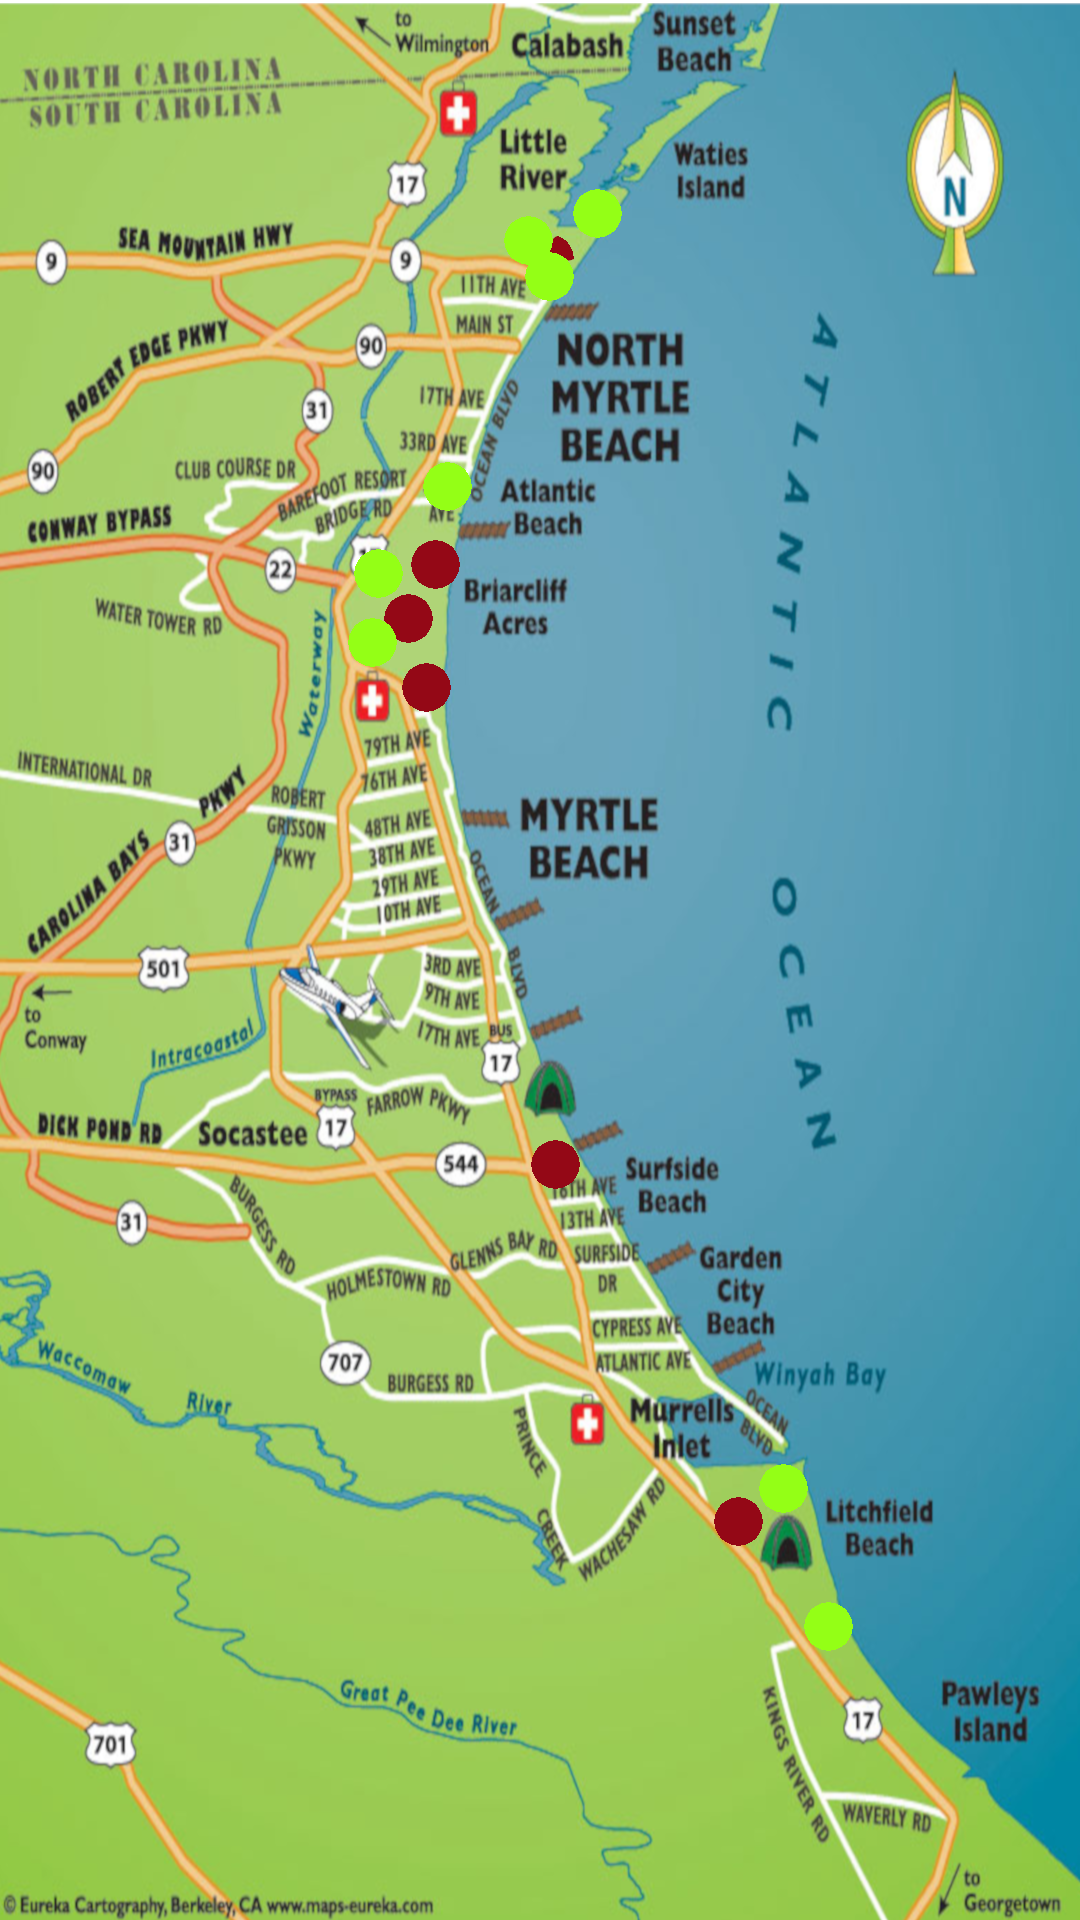
\includegraphics[width=\textwidth]{mock1.png}

\end{minipage}

\begin{minipage}{\textwidth}

{\huge Rent component}

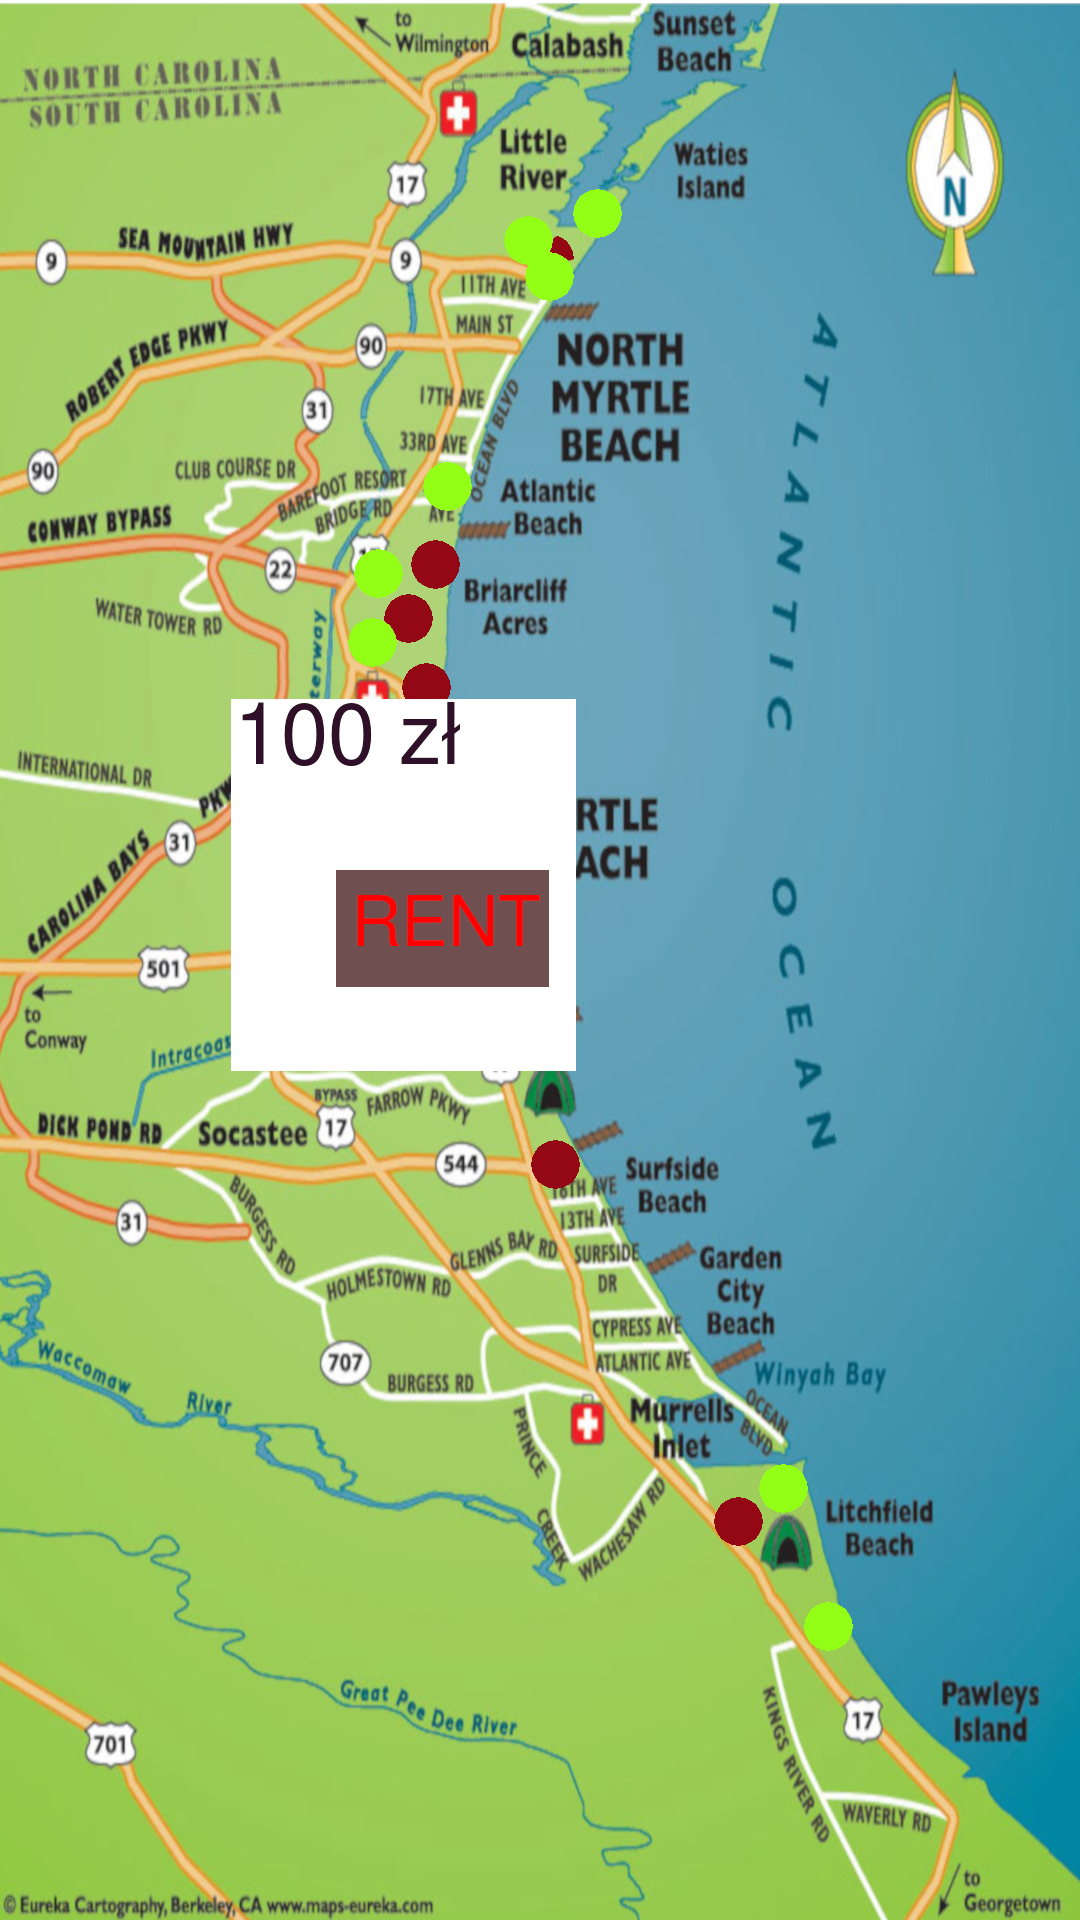
\includegraphics[width=\textwidth]{mock2.png}

\end{minipage}

\begin{minipage}{\textwidth}

{\huge Login view}

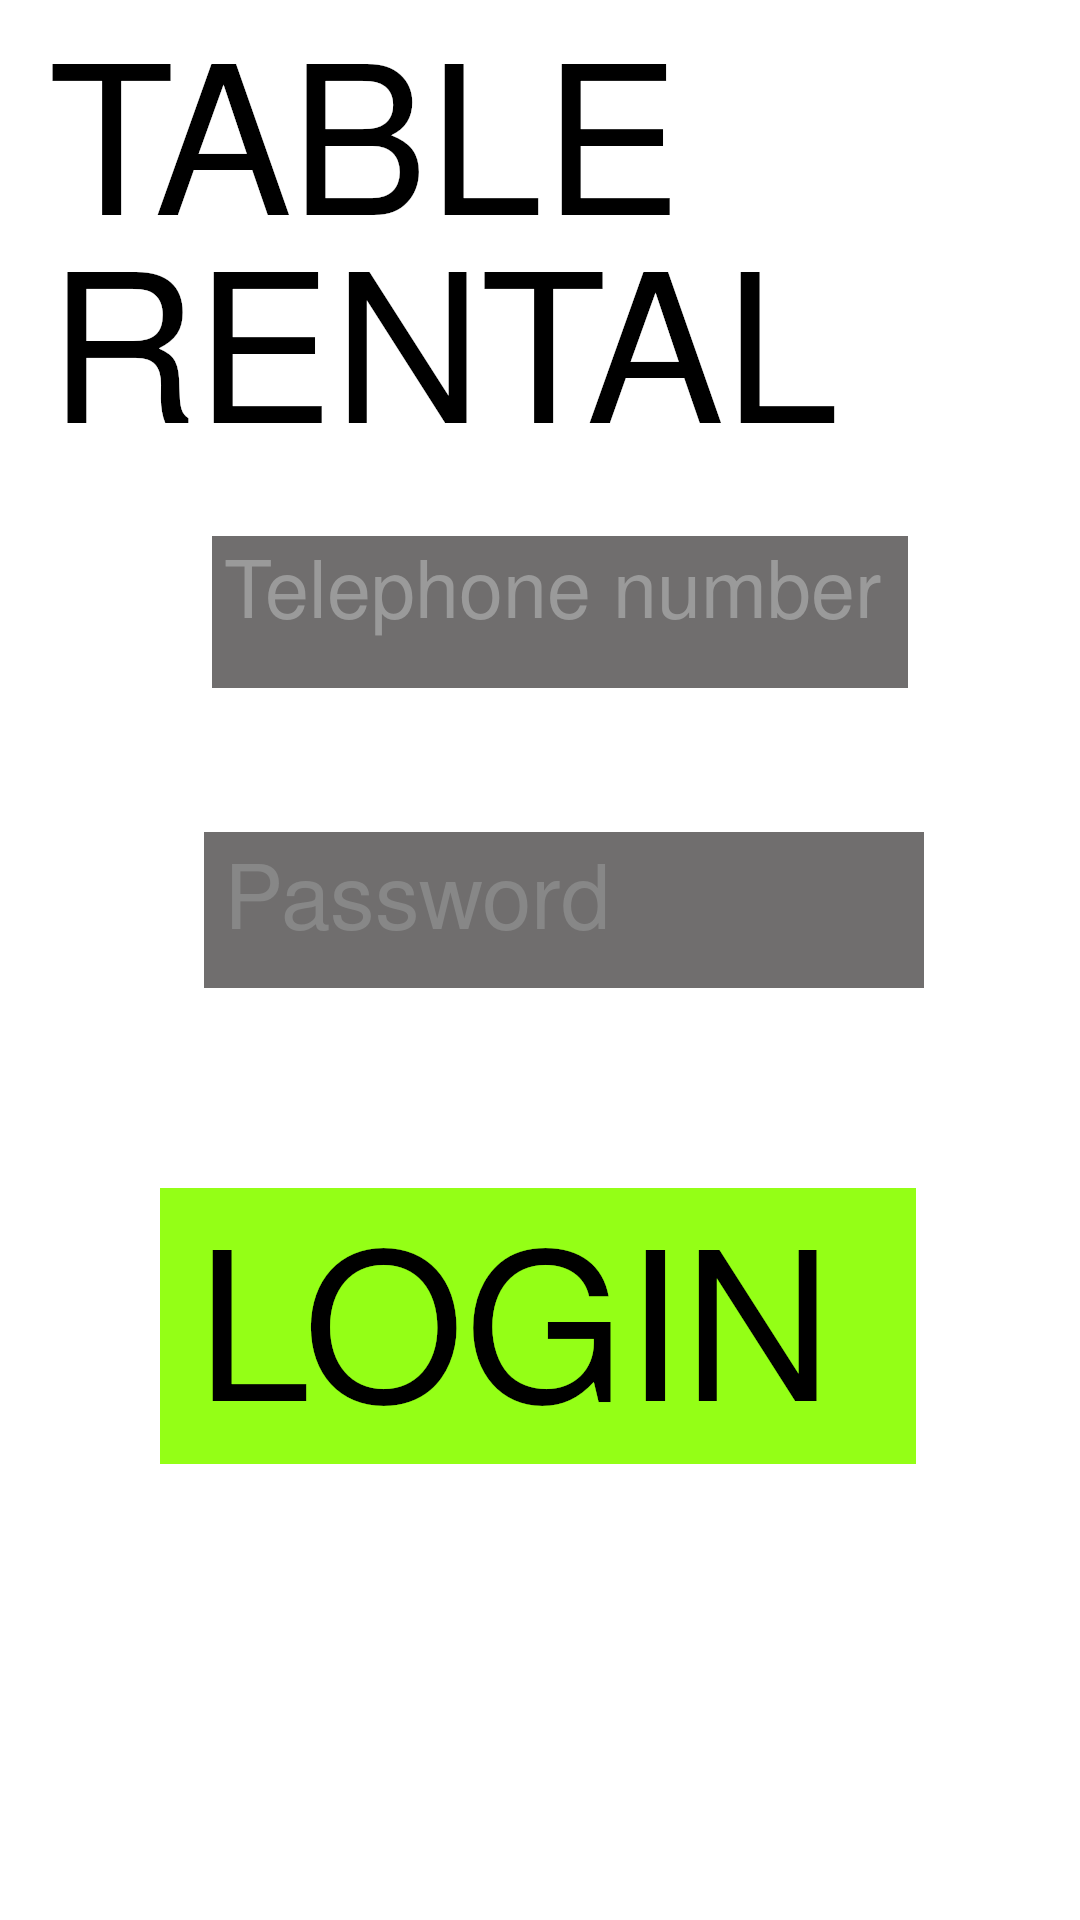
\includegraphics[width=\textwidth]{mock3.png}

\end{minipage}


\subsubsection{Software Interface}

Web frontend will be communicating with backend through REST API.
\section{System Features}
\subsection{Authentication}
\subsubsection{Registration}
User should be able to register with their phone number, or Facebook account.
\subsubsection{Login}
User should be able to log in into the Application with their phone number, or Facebook account.
\subsection{Map}
\subsubsection{Occupated/unoccupated tables}
User should be able to see a map in the Application, indicating the position of Tables. The Tables should be marked green/red in case their are unoccupied/occupied.
\subsubsection{Clicking on a table icon}
When user clicks on a table icon on the Map he/she should be provided with informations like:
\begin{itemize}
    \item In which hours the Table will be free.
    \item What's the prica of table rental.
\end{itemize}
\subsection{Renting}
User should be able to click "Rent" button after clicking on a Table icon, then he/she should be provided with avaliable method payments.
\subsection{Malcious usage}
It the User, who rented the Table notices it is being occupated illegally by malcious user, he/she should be able to call, with a single click in the application, battle robots, which will be responsible for transporting the malcious users away, so the right Table notices it is being occupated illegally by malcious user, he/she should be able to call, with a single click in the application, battle robots, which will be responsible for transporting the malcious users away, so the right Table owner is able to use it.
\end{document}
